\chapter{Introduction}\label{ch:intro}

Since its development in the 1970s, the Standard Model of particle physics has been an enormously successful description of observed phenomena, withstanding many precision tests. However, despite this success, it is widely believed to be incomplete. Among its shortcomings is the hierarchy problem, which arises due to the large difference between two fundamental scales in the theory. The existence of extra spatial dimensions in the universe has been proposed as one possible solution to this problem. This dissertation aims to address this issue by searching for evidence of large extra dimensions at the Large Hadron Collider using proton-proton collisions at the energy frontier.

\section{Standard Model}

The Standard Model (SM) of particle physics is a gauge theory describing the dynamics of the known fundamental particles and their interactions through the strong, weak, and electromagnetic forces (with the notable exception of gravity). A gauge theory is a quantum field theory in which the Lagrangians describing the evolution and interactions of the particles remain invariant under local transformations of a symmetry group. Particles are described as excitations of quantum fields in (3\texttt{+}1)-dimensional spacetime whose properties are defined by their representations under different symmetry groups. There are two types of particles: bosons, which have integer spin with symmetric wave functions under the exchange of two identical particles, and fermions, which have half-integer spin with antisymmetric wave functions under identical particle exchange. Fermions are the matter particles and their interactions are mediated by bosons, the force carriers.

Gauge theories based on the special unitary group of degree $\mathrm{N}$, $\mathrm{SU}(\mathrm{N})$, are known as Yang-Mills theories~\cite{Yang:1954ek}. The SM is the Yang-Mills theory of the gauge group %$\mathrm{SU}(3)_c \times \mathrm{SU}(2)_L \times \mathrm{U}(1)_Y$.
\begin{equation*}
	\mathrm{SU}(3)_c \times \mathrm{SU}(2)_L \times \mathrm{U}(1)_Y
\end{equation*}
The group $\mathrm{SU}(3)_c$ corresponds to the strong force and $\mathrm{SU}(2)_L \times \mathrm{U}(1)_Y$ to the unification of the electromagnetic and weak forces, known as the electroweak force. The gauge transformation of $\mathrm{SU}(3)_c$ yields the fields $G_{\mu}^{\alpha}$, for $\alpha = 1$, 2, \dots, 8; $\mathrm{SU}(2)_L$ yields $W_{\mu}^a$, for $a = 1$, 2, 3; and $\mathrm{U}(1)_Y$ yields $B_{\mu}$, where $\mu$ is the component in (3\texttt{+}1)-dimensions. These gauge fields give rise to gauge bosons, which are also the generators of the group. These gauge bosons are the 8 gluons ($g$) for $\mathrm{SU}(3)_c$ and the $W^{\pm}$ and $Z$ bosons and photon ($\gamma$) for $\mathrm{SU}(2)_L \times \mathrm{U}(1)_Y$. These are all vector (spin-1) gauge bosons. The gauge bosons $W^{\pm}$, $Z$, and $\gamma$ are obtained after electroweak symmetry breaking, as discussed below. The gluons mediate the strong force, the $W^{\pm}$ and $Z$ bosons mediate the weak force, and the photon mediates the electromagnetic force.

Fermion fields are associated with every observed matter particle. These are spin-1/2 fermions that exist in two varieties: quarks, which participate in the strong interaction, and leptons, which do not. For each \correction{charged} fermion there is also a corresponding antifermion of the same mass but opposite electric charge. There are three generations of the fermions, which are identical except for the associated particle masses between generations. Each generation contains an up-type quark, a down-type quark, a charged lepton, and a neutral lepton, called a neutrino. The up-type quarks have an electric charge of $+\frac{2}{3}$ and are the up ($u$), charm ($c$), and top ($t$) quarks. The down-type quarks have an electric charge of $-\frac{1}{3}$ and are the down ($d$), strange ($s$), and bottom ($b$) quarks. The charged leptons have an electric charge of $-1$ and are the electron ($e^-$), muon ($\mu^-$), and tau ($\tau^-$). The neutrinos are electrically neutral and are the electron neutrino ($\nu_e$), muon neutrino ($\nu_{\mu}$), and tau neutrino ($\nu_{\tau}$). Each fundamental particle is assigned to a particular representation of the SM gauge group.

Each flavor of quark transforms under the fundamental representation ($\mathbf{3}$) of $\mathrm{SU}(3)_c$, forming ``color" triplets. \correction{Each quark has a color charge} (as denoted by the subscript $c$) of red, green, or blue. (Antiquarks have a color charge of antired, antigreen, or antiblue.) By analogy with the three primary colors of light, the quark triplets contain a red, green, and blue charged quark state. The leptons are assigned to the trivial representation ($\mathbf{1}$) of $\mathrm{SU}(3)_c$, forming color singlets. Particles represented as singlets under any symmetry group remain unchanged by the associated transformation and, hence, are not influenced by the corresponding interaction. The left-handed ($L$) chiral components of the fermions are grouped into $\mathrm{SU}(2)_L$ weak doublets, transforming under its fundamental representation ($\mathbf{2}$). The right-handed fermions are $\mathrm{SU}(2)_L$ weak singlets with the trivial representation ($\mathbf{1}$). \correction{There are no right-handed neutrinos in the simplest form of the theory.} The hypercharge ($Y$) describes the fermion coupling to $\mathrm{U}(1)_Y$, chosen to reproduce the electrical charges of the particles. The electrical charge $Q_{\mathrm{EM}} = T^3 + \frac{Y}{2}$, where $T^3$ is the third component of the weak isospin. These representations are summarized in Table~\ref{tab:fermion_representations}.

\begin{table}[!htbp]
	\caption{The representations of a single generation of fermions in the SM gauge group. The ordered triplets correspond to their representations under the groups ordered as ($\mathrm{SU}(3)_c$, $\mathrm{SU}(2)_L$, $\mathrm{U}(1)_Y$). Here, the generic symbols $e$ and $\nu$ are used to denote the charged and neutral leptons, respectively, and $u$ and $d$ for the up- and down-type quarks, respectively. The left- and right-handed fermions are separated using the respective subscripts $L$ and $R$.}
	\centering
	\vspace{\baselineskip}
	\begin{tabular}{cccccc}
		\hline \hline
		\vspace*{-4.0mm} & & & & & \\
		SM fermion & $q_L = \begin{pmatrix} u_L \\ d_L \end{pmatrix}$ & $u_R$ & $d_R$ & $\ell_L = \begin{pmatrix} \nu_L \\ e_L \end{pmatrix}$ & $e_R$ \\
		\vspace*{-4.0mm} & & & & & \\
		\parbox{5cm}{\centering ($\mathrm{SU}(3)_c$, $\mathrm{SU}(2)_L$, $\mathrm{U}(1)_Y$) \\ representation} & $(\mathbf{3},\mathbf{2},\frac{1}{6})$ & $(\mathbf{3},\mathbf{1},\frac{2}{3})$ & $(\mathbf{3},\mathbf{1},-\frac{1}{3})$ & $(\mathbf{1},\mathbf{2},-\frac{1}{2})$ & $(\mathbf{1},\mathbf{1},-1)$ \\
		\vspace*{-4.0mm} & & & & & \\
		\hline \hline
	\end{tabular}
	\label{tab:fermion_representations}
\end{table}

The gluons belong to the adjoint representation ($\mathbf{8}$) of $\mathrm{SU}(3)_c$, forming color octets. Gluons carry color-anticolor pairs with their eight states given as combinations of these pairs. The gauge boson fields $G_{\mu}^{\alpha}$, $W_{\mu}^a$, and $B_{\mu}$ have the representations $(\mathbf{8},\mathbf{1},0)$, $(\mathbf{1},\mathbf{3},0)$, and $(\mathbf{1},\mathbf{1},0)$, respectively, corresponding the groups ordered as ($\mathrm{SU}(3)_c$, $\mathrm{SU}(2)_L$, $\mathrm{U}(1)_Y$). Gauge invariance prohibits explicit mass terms in the Lagrangians for the gauge bosons. Indeed, the gluons and photon are massless; however, the $W^{\pm}$ and $Z$ bosons have masses of approximately 80 and 91\GeV\footnote{The convention in particle physics is to use natural units with $\hbar = c = 1$. Hence, energy, momentum, and mass, which have the respective units of {\eVns}, ${\eVns}/c$, and ${\eVns}/c^2$, are all given in units of {\eVns}.}. This problem is circumvented through the realization that the ground state, or vacuum, of the theory does not need to exhibit the same symmetries as the Lagrangian. This is known as spontaneous symmetry breaking and underlies the Higgs mechanism~\cite{Englert:1964et,Higgs:1964ia,Higgs:1964pj,Guralnik:1964eu,Higgs:1966ev,Kibble:1967sv}.

The spontaneous breaking of a continuous global symmetry implies the existence of massless scalar (spin-0) bosons called Goldstone bosons~\cite{Nambu:1960tm,Goldstone:1961eq,Goldstone:1962es}. However, when the symmetry is local, the spontaneous breaking causes the Goldstone bosons to disappear and the Goldstone modes result in the gauge bosons associated with the broken symmetry to become massive through the Higgs mechanism. The Higgs mechanism introduces a Higgs field, which is a complex scalar field that transforms as a doublet under $\mathrm{SU}(2)_L$. The Higgs field has the representation $(\mathbf{1},\mathbf{2},\frac{1}{2})$ under the groups ordered as ($\mathrm{SU}(3)_c$, $\mathrm{SU}(2)_L$, $\mathrm{U}(1)_Y$). The spontaneous symmetry breaking of the electroweak gauge group $\mathrm{SU}(2)_L \times \mathrm{U}(1)_Y$ to the quantum electrodynamic (QED) gauge group $\mathrm{U}(1)_{\mathrm{EM}}$ results in the $W^{\pm}$ and $Z$ bosons acquiring mass. The vacuum is invariant under $\mathrm{U}(1)_{\mathrm{EM}}$ transformations, allowing the photon to remain massless. This mechanism also predicts a massive, electrically neutral scalar boson, called the Higgs ($H$) boson. This boson was recently discovered by the ATLAS and CMS Collaborations, having mass near 125\GeV with properties consistent with the SM prediction~\cite{Aad:2012tfa,Chatrchyan:2012xdj,Aad:2015zhl,Khachatryan:2016vau,Sirunyan:2018koj}.

The Higgs mechanism can also explain the presence of fermion masses. Since the weak interaction violates parity, it couples differently to left- and right-handed fermions. Fermion mass terms in the Lagrangian would arise by coupling these separate fields, but this would break $\mathrm{SU}(2)_L$ gauge invariance. Thus, fermions should appear massless in nature, a contradiction with observation. In contrast to the mass generation for the massive gauge bosons, the fermions acquire mass through Yukawa interactions with the Higgs field. The strength of the Yukawa coupling for a fermion to the Higgs boson is directly proportional to its mass. \correction{Despite the absence of right-handed neutrinos in the simplest form of the theory, neutrino oscillation experiments have demonstrated that neutrino masses are nonzero and mix among their three flavor eigenstates, as discussed in Section~63 or Ref.~\cite{Tanabashi:2018oca}. The mechanism for generating neutrino masses has not been established.} A summary of the SM particles, including their masses, is given in Table~\ref{tab:SM_particles}.

\begin{table}[!htb]
	\centering
	\caption{A list of the SM particles, each with their corresponding mass, spin, and charge. The masses are approximated from Ref.~\cite{Tanabashi:2018oca}. The electric charge is given in units of $e$, the elementary charge. \correction{Due to the large mixing in the neutrino sector, the mass differences between the different neutrino flavors are small and it's difficult to refer to individual neutrino mass eigenstates. Since the mass measurement of $\nu_e$ is the most stringent among the different neutrino flavors, the masses of $\nu_{\mu}$ and $\nu_{\tau}$ have been constrained by it.}}
	\vspace{\baselineskip}
	\begin{tabular}{c|ccc}
	\hline \hline
	Particle       & Mass & Spin & Charge \\
	\hline
	$u$ & 2.2\MeV   & 1/2 & +2/3 \\
	$d$ & 4.7\MeV   & 1/2 & -1/3 \\
	$c$ & 1.275\GeV & 1/2 & +2/3 \\
	$s$ & 95\MeV    & 1/2 & -1/3 \\
	$t$ & 173\GeV   & 1/2 & +2/3 \\
	$b$ & 4.18\GeV  & 1/2 & -1/3 \\
	\hline
	$e^-$        & 0.511\MeV    & 1/2 & -1 \\
	$\nu_e$      & $< 2\eV$     & 1/2 & 0  \\
	$\mu^-$      & 106\MeV      & 1/2 & -1 \\
	$\nu_{\mu}$  & \correction{$< 2\eV$} & 1/2 & 0  \\ % $\nu_{\mu}$  & $< 0.19\MeV$ & 1/2 & 0  \\
	$\tau^-$     & 1.78\GeV     & 1/2 & -1 \\
	$\nu_{\tau}$ & \correction{$< 2\eV$} & 1/2 & 0  \\ % $\nu_{\tau}$ & $< 18.2\MeV$ & 1/2 & 0  \\
	\hline
	$\gamma$   & 0           & 1 & 0    \\
	$W^{\pm}$  & 80.4\GeV    & 1 & $\pm1$ \\
	$Z$        & 91.1876\GeV & 1 & 0    \\
	$g$        & 0           & 1 & 0    \\
	$H$        & 125.18\GeV  & 0 & 0    \\
	\hline \hline
	\end{tabular}
	\label{tab:SM_particles}
\end{table}

The theory of quantum chromodynamics (QCD) describes the interactions of the quarks under the strong force, based on the non-Abelian gauge group $\mathrm{SU}(3)_c$. \correction{At low energies, free quarks are not observed} and, instead, become confined to hadrons, which are composite particles made up of quarks. Hadrons made up of three quarks are called baryons and those made up of a quark-antiquark pair are called mesons. There are also hadrons containing more than three valence quarks. Experimental measurements have shown that the energy scale at which QCD becomes confining is $\Lambda_{\mathrm{QCD}} \approx 300\MeV$~\cite{Halzen:1984mc,Tanabashi:2018oca}. At high energies, however, QCD has a perturbative regime as the strength of the strong interaction becomes small, allowing quarks and gluons to behave as nearly free particles. This behavior is called asymptotic freedom and was demonstrated by Politzer, Gross, and Wilczek~\cite{Gross:1973id,Politzer:1973fx}.

Asymptotic freedom is a particular case of the more general phenomenon of running coupling constants, where the values of the coupling constants change depending on the energy scale of the interaction ($Q$) due to the participation of virtual particles in the interaction. These virtual particles can lead to infinities through loops in the Feynman diagrams during the calculation. Reparameterizing the bare parameters into physical parameters absorbs the divergences and leads to finite and measurable effects. This process is known as renormalization~\cite{tHooft:1972tcz} and introduces the (unphysical) renormalization scale. Once the value of the coupling constant is known at this scale, its dependence on $Q$ can be determined. At $Q \approx 100\GeV$, the strong coupling constant $\alpha_s \approx 0.1$. This is in contrast to that of the QED coupling constant, $\alpha_{\mathrm{EM}}$, which increases as $Q$ increases due to charge screening from vacuum polarization. In QCD, its non-Abelian nature results in gluons carrying color, which causes the effective color charge to be spread out in the vacuum. The asymptotic value of $\alpha_{\mathrm{EM}} \approx 1/137$.

The gauge structure of the electroweak theory with gauge group $\mathrm{SU}(2)_L \times \mathrm{U}(1)_Y$ was proposed by Glashow, Weinberg, and Salam~\cite{Glashow:1961tr,Weinberg:1967tq,Salam:1968rm}. The combination of the electroweak and QCD theories became known as the SM. All of the ideas presented here about the SM can be summarized in Lagrangian form. The SM Lagrangian density (see, e.g., Ref.~\cite{Halzen:1984mc}), given in terms of the particle fields and their couplings, is
\begin{align}
	\mathcal{L} = &-\frac{1}{4} G_{\mu\nu}^{\alpha}G^{\alpha\mu\nu} -\frac{1}{4} W_{\mu\nu}^aW^{a\mu\nu} -\frac{1}{4} B_{\mu\nu}B^{\mu\nu} \nonumber \\
				  &+\bar{q}_L i \slashed{D} q_L + \bar{u}_R i \slashed{D} u_R + \bar{d}_R i \slashed{D} d_R \nonumber \\
				  &+\bar{\ell}_L i \slashed{D} \ell_L + \bar{e}_R i \slashed{D} e_R \label{eqn:SM_langrangian} \\
				  &+(D_{\mu}\phi)^{\dagger}(D^{\mu}\phi) - V(\phi) \nonumber \\
				  &-y_u\bar{q}_L \tilde{\phi} u_R - y_d\bar{q}_L \phi d_R - y_e\bar{\ell}_L \phi e_R \nonumber
\end{align}
where $G_{\mu\nu}^{\alpha}$, $W_{\mu\nu}^a$, and $B_{\mu\nu}$ are the gauge field-strength tensors, which are defined in terms of the gauge fields, $G_{\mu}^{\alpha}$, $W_{\mu}^a$, and $B_{\mu}$, respectively; $\slashed{D} = D_{\mu}\gamma^{\mu}$, where $\gamma^{\mu}$ are the Dirac matrices and $D_{\mu}$ is the gauge-covariant derivative; $\phi$ is the Higgs field; $V(\phi)$ is the Higgs potential; $\tilde{\phi} = i\sigma_2\phi^{*}$, where $\sigma_a$ are the $2{\times}2$ Pauli matrices; and $y_u$, $y_d$, and $y_e$ are the Yukawa couplings of the associated up-type quark, down-type quark, and charged lepton. Each Yukawa coupling is directly related to the corresponding fermion mass. The hermitian conjugate of the three terms with Yukawa couplings are also considered in this equation, but not explicitly listed. The gauge-covariant derivative $D_{\mu} = \partial_{\mu} - \frac{i}{2}g_s\tau_{\alpha}G_{\mu}^{\alpha} - \frac{i}{2}g\sigma_aW_{\mu}^a - \frac{i}{2}g^{\prime}YB_{\mu}$, where $\tau_{\alpha}$ are the $3{\times}3$ Gell-Mann matrices and $g_s$, $g$, and $g^{\prime}$ are the gauge coupling constants associated with $\mathrm{SU}(3)_c$, $\mathrm{SU}(2)_L$, $\mathrm{U}(1)_Y$, respectively. If any particle (fermion or Higgs) field is a singlet under one of the SM gauge groups, then the term in $D_{\mu}$ involving the corresponding gauge boson field of that gauge group is omitted. The coupling $g_s$ is directly proportional to $\alpha_s$ and both $g$ and $g^{\prime}$ can be related to $\alpha_{\mathrm{EM}}$. The gauge couplings $g$ and $g^{\prime}$ are also related to the masses of the $W^{\pm}$ and $Z$ bosons and, among others, including the Yukawa couplings, are free parameters in the theory.

Gauge invariance restricts the form of the terms in the SM Lagrangian, which determine the possible particle interactions by constraining their couplings. The first line in Eq.~(\ref{eqn:SM_langrangian}) describes the kinetic energies and self-interactions of the gauge bosons; the second and third lines describe the kinetic energies and electroweak interactions of the fermions, as well as the strong interactions between the quarks and gluons; the forth line describes the electroweak and Higgs boson masses and couplings; and the fifth line describes the fermion masses and their couplings to the Higgs boson. \correction{Since the mechanism for generating the neutrino masses has not been established, no term has been added to Eq.~(\ref{eqn:SM_langrangian}) to explain this.} The interactions between the fermions and the vector gauge bosons are depicted in the Feynman diagrams shown in Fig.~\ref{fig:SM_interactions}. The electroweak bosons are allowed to have cubic and quartic couplings of the form $WW\gamma$, $WWZ$, $WWWW$, $WW\gamma\gamma$, $WWZZ$, and $WWZ\gamma$. Since gluons carry color and, hence, can self-interact, the cubic and quartic couplings of the form $ggg$ and $gggg$ are possible. The Higgs boson couples to massive SM bosons or fermions and can also self-interact. The Higgs boson cubic and quartic couplings among the SM bosons are of the form $HWW$, $HZZ$, $HHH$, $HHWW$, $HHZZ$, and $HHHH$. Feynman diagrams depicting the Higgs boson interactions among the SM gauge bosons and fermions are shown in Fig.~\ref{fig:higgs_interactions}.

\begin{figure}[!htb]
	\centering
	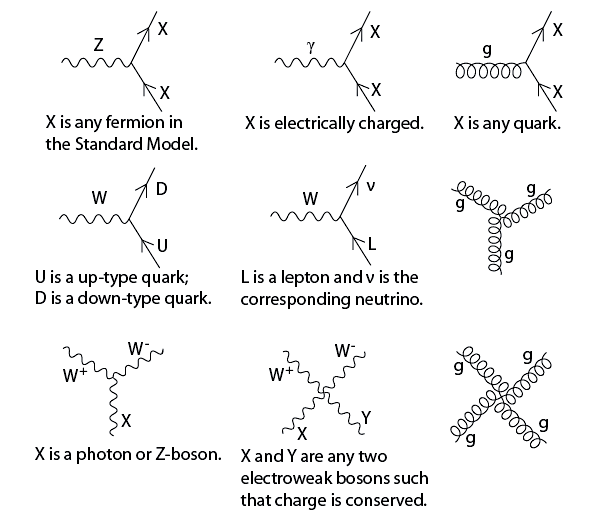
\includegraphics[width=0.84\textwidth]{figures/Standard_Model_Feynman_Diagram_Vertices.png}
	\caption{Feynman diagrams representing the interactions between the fermions and vector gauge bosons in the SM~\cite{SM_interactions}. The charges of the $W$ bosons are determined by conserving charge with the fermions they interact with.}
	\label{fig:SM_interactions}
\end{figure}

\begin{figure}[!htb]
	\centering
	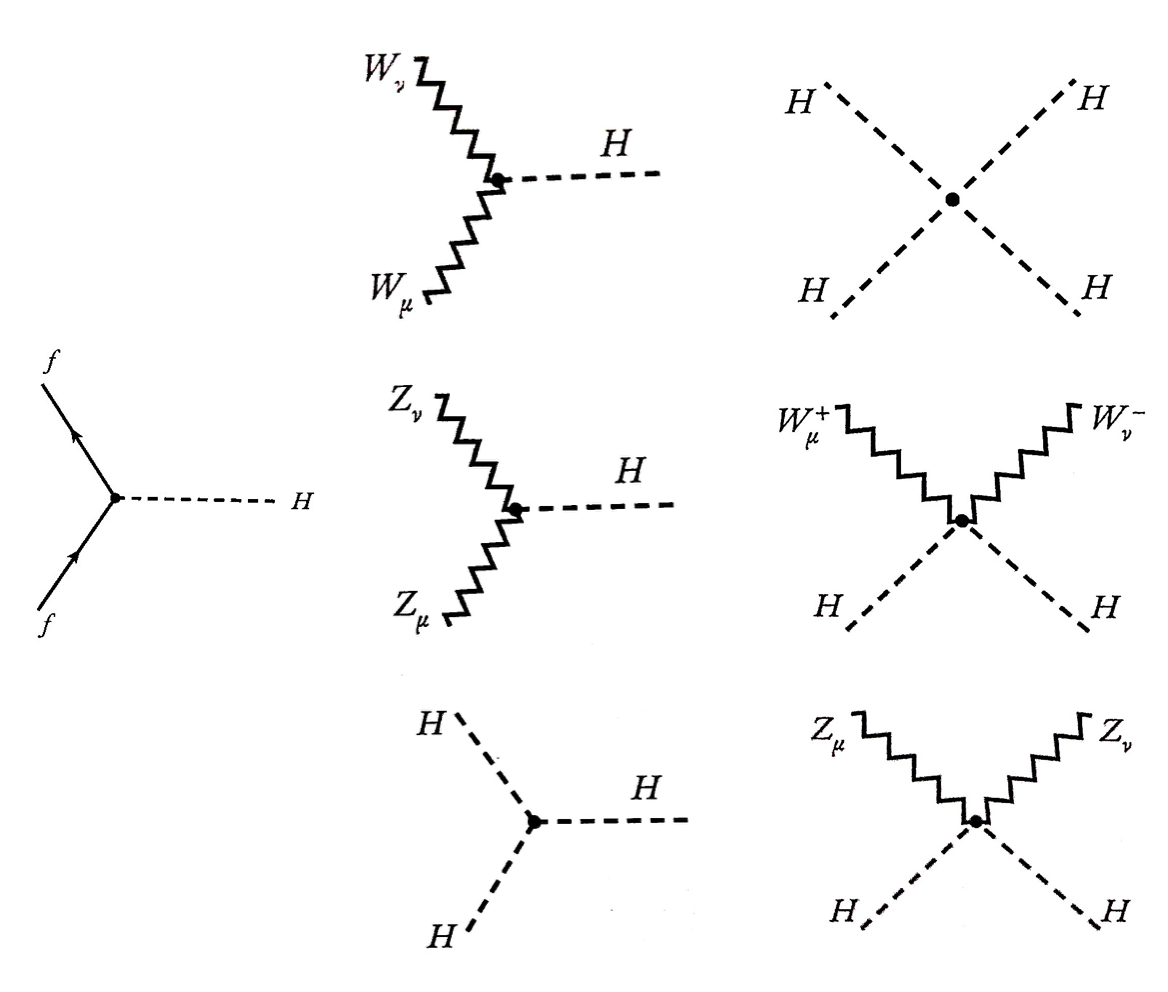
\includegraphics[width=0.75\textwidth]{figures/higgs_sm_couplings.png}
	\caption{Feynman diagrams representing the Higgs boson interactions with the fermions ($f$) and gauge bosons in the SM~\cite{Quigg:2013ufa}.}
	\label{fig:higgs_interactions}
\end{figure}

One mechanism for studying the SM predictions and measuring its free parameters is through particle collisions. At the energy frontier, the SM is currently being probed from proton-proton collisions at the Large Hadron Collider (LHC). Protons are baryons made up of three valence quarks (two $u$ quarks and one $d$ quark), gluons, and sea quarks. Any single proton-proton collision actually involves the interactions among its partons, with the largest momentum transfer occurring in the hard parton-parton collision. The distribution among the partons within the protons is determined from experiment and described by parton distribution functions, which will be used and further discussed in Chapter~\ref{ch:background}. 

The success of the SM can be seen in Fig.~\ref{fig:cms_sm_xsec}, which shows excellent agreement between a wide range of theory and experimental cross section measurements, spanning several orders of magnitude, for the production of various SM processes, as measured by the CMS Collaboration at the LHC. Despite its success, there are several observations not described by the SM. These include a lack of description for dark matter (Section~26, Ref.~\cite{Tanabashi:2018oca}), dark energy (Section~27, Ref.~\cite{Tanabashi:2018oca}), neutrino mass (Section~14, Ref.~\cite{Tanabashi:2018oca}), matter-antimatter asymmetry (Section~21, Ref.~\cite{Tanabashi:2018oca}), vacuum stability (Section~11, Ref.~\cite{Tanabashi:2018oca}), and gravity. In addition, there are several theoretical issues, including no explanation for the large number of free parameters (including why the Yukawa couplings range over six orders of magnitude, or why there are three generations or fermions), no evidence of strong CP violation (Section~13, Ref.~\cite{Tanabashi:2018oca}), no understanding of the origin of gauge group unification, and no solution to the hierarchy problem~\cite{hp1,hp2}. A large number of theories have been developed to solve these issues, such as supersymmetry (Sections~109 and~110, Ref.~\cite{Tanabashi:2018oca}), leptoquarks (Section~115, Ref.~\cite{Tanabashi:2018oca}), and extra-dimensional models (Section~106, Ref.~\cite{Tanabashi:2018oca}). We will investigate the SM hierarchy problem and look at its proposed solution through the addition of extra spatial dimensions in the universe.

\begin{figure}[!htb]
  \centering
  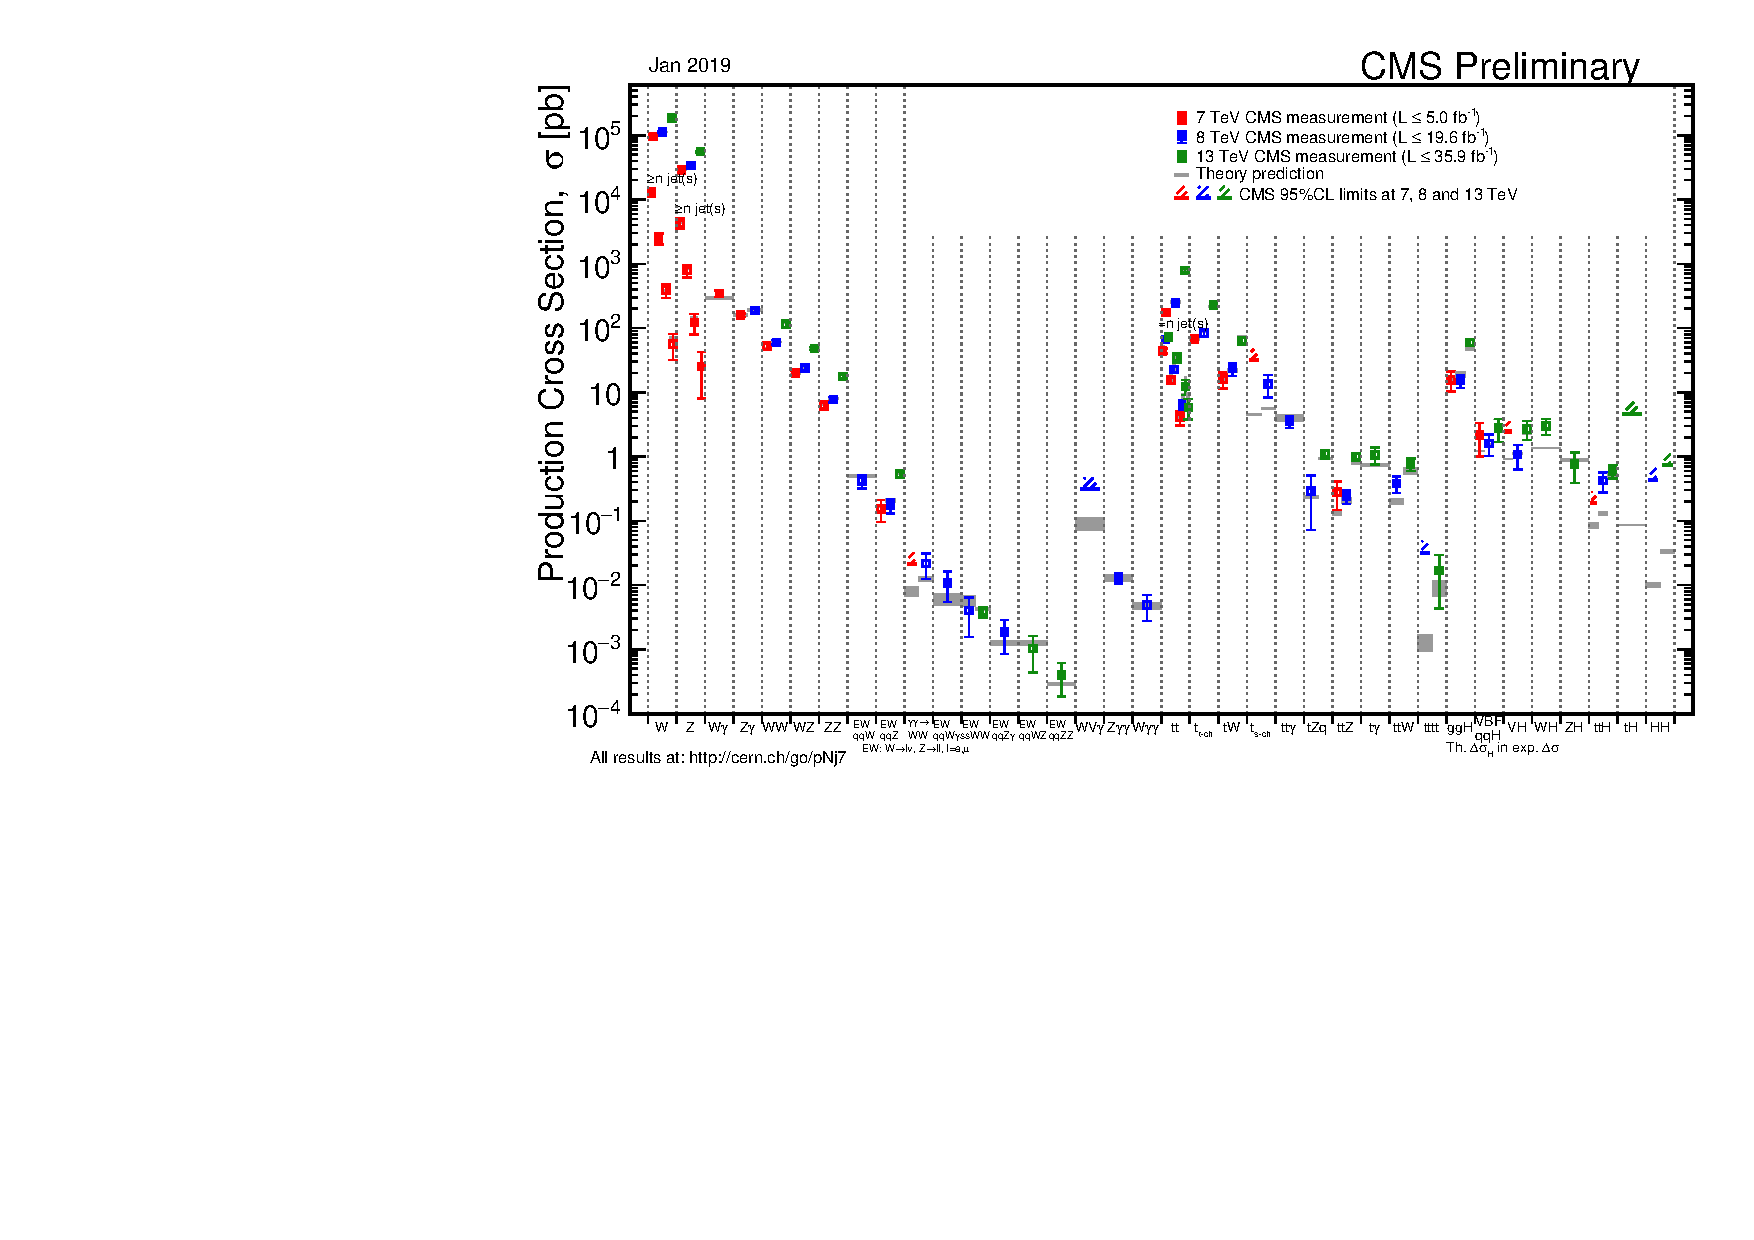
\includegraphics[width=1.0\textwidth]{figures/cms_sm_xsec}
  \caption{Summary of the theory and experimental production cross section measurements of SM processes, measured by the CMS Collaboration~\cite{CMS_xsec}.}
  \label{fig:cms_sm_xsec}
\end{figure}


\section{Beyond the Standard Model}

The shortcomings of the Standard Model suggest that there exists new physics beyond the Standard Model (BSM), offering solutions to its issues. The hierarchy problem, in particular, could be resolved by the existence of extra spatial dimensions in the universe. Among the various extra-dimensional models, the model of large extra dimensions is the focus of this dissertation.

\subsection{Hierarchy Problem}

The hierarchy problem~\cite{hp1,hp2} arises from the large difference between the electroweak scale, $M_{\mathrm{EW}} \sim 10^2\GeV$, and the Planck scale, $\Mpl = (\hbar c/G_{\mathrm{N}})^{1/2} \sim 10^{19}\GeV$, where $G_{\mathrm{N}}$ is Newton's gravitational constant, and has consequences related to the Higgs boson mass $m_H$. Since the Higgs boson is a scalar, coupling to mass, it receives large quantum corrections proportional to $\Lambda^2$ for an ultraviolet cutoff scale $\Lambda$ up to where the theory is valid. This scale arises during the integration of the undetermined momenta of the virtual particles in the loop diagrams associated with the quantum corrections and is used to regulate the loop integrals. Since the Higgs boson is the only scalar in the SM, it is the only SM particle not protected from these corrections. The corrections to the physical Higgs boson mass are of the form
\begin{equation}
	m_H^2 = m_0^2 + \Delta m_H^2
\end{equation}
where $m_0$ is the bare Higgs boson mass and $\Delta m_H^2$ are the mass contributions from the radiative corrections. The one-loop corrections due to a fermion $f$ with Yukawa coupling $y_f$ are given by
\begin{equation}
	m_H^2 \approx m_0^2 - \frac{|y_f|^2}{8\pi^2}\Lambda^2
\end{equation}
The contribution from the $t$ quark is largest with coupling $y_t \sim 1$. The dominant one-loop corrections come from the massive gauge bosons, Higgs boson self-coupling, and the $t$ quark and contribute~\cite{Quigg:2013ufa}
\begin{equation}
	\Delta m_H^2 = \frac{G_F \Lambda^2}{4 \pi^2 \sqrt{2}} (6m_W^2 + 3m_Z^2 + m_H^2 - 12m_t^2)
\end{equation}
where $m_W$, $m_Z$, and $m_t$ are the masses of the $W$ boson, $Z$ boson, and $t$ quark, respectively; and $G_F$ is the Fermi constant, which can be related to each particle's coupling constant. The Feynman diagrams depicting these one-loop corrections are shown in Fig.~\ref{fig:higgs_corrections}.  

\begin{figure}[!htb]
	\centering
	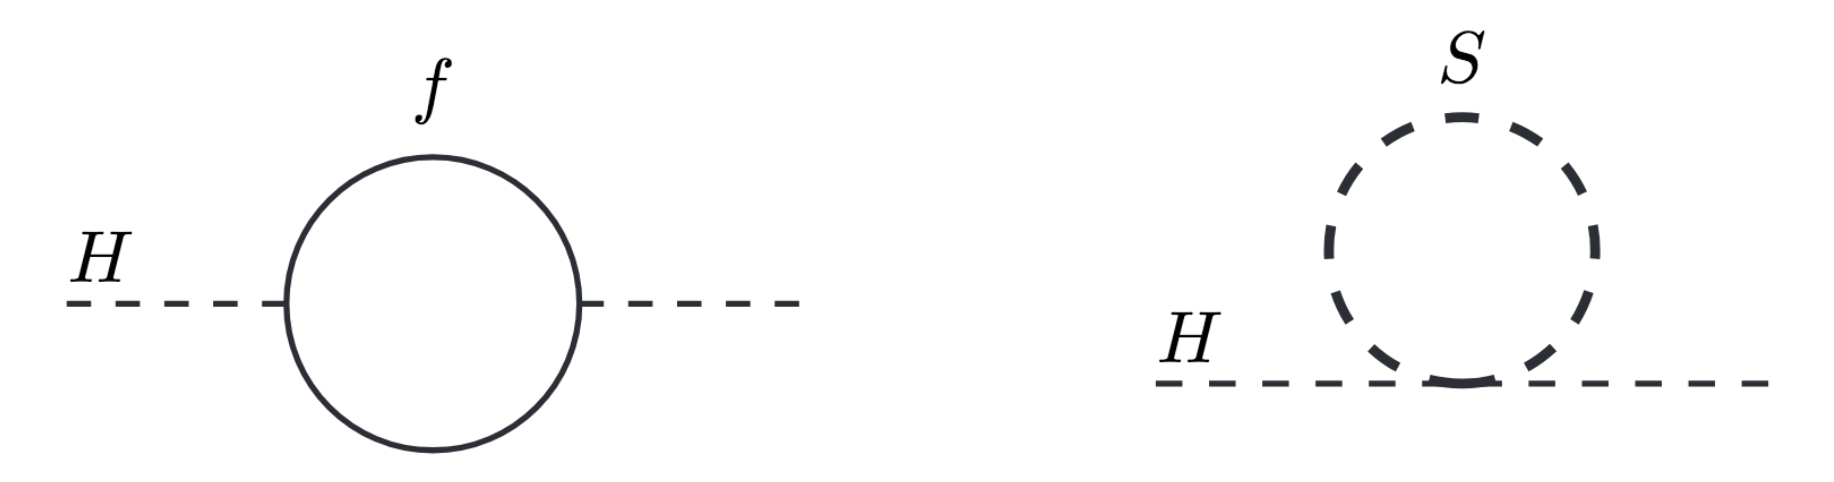
\includegraphics[width=0.75\textwidth]{figures/higgs_corrections.png}
	\caption{One-loop Feynman diagrams for the quantum corrections to the Higgs boson squared mass due to fermions (left) and bosons (right)~\cite{Martin:1997ns}.}
	\label{fig:higgs_corrections}
\end{figure}

The only candidate reference scale for $\Lambda$ is the Planck scale, at which quantum gravity is expected to emerge. Using this scale, the bare mass and the quantum corrections would have to cancel over 30 orders of magnitude in order to arrive at the experimental value of $m_H \simeq 125\GeV$. This extreme degree of cancellation is referred to as fine tuning and seems unnatural. This suggests the possibility of new physics BSM that acts to preserve $m_H$, eliminating the fine tuning requirement. Many models have been proposed. We consider the addition of extra spatial dimensions in the universe as a possible solution, realized through their modification of the fundamental Planck scale.


\subsection{Large Extra Dimensions}

There are several extra-dimensional models that exist since the original idea by Kaluza and Klein~\cite{Kaluza:1921tu,Klein:1926fj,Klein:1926tv}. Among these are the model by Arkani-Hamed, Dimopoulos, and Dvali (ADD)~\cite{ArkaniHamed:1998rs,Antoniadis:1998ig,ArkaniHamed:1998nn}, which proposes flat, large extra dimensions, and the model by Randall and Sundrum~\cite{Randall:1999ee,Randall:1999vf}, which proposes a single, warped extra dimension. A general review of extra-dimensional models and their experimental searches can be found in Section~106 of Ref.~\cite{Tanabashi:2018oca} or in the summary by Hewett and Spiropulu~\cite{Hewett:2002hv}. In general, these models modify the fundamental Planck scale, \MD, such that it can be much lower than the observed Planck scale, \Mpl. In fact, \MD can be on the order of $M_{\mathrm{EW}}$, which would solve the hierarchy problem. Not only could these models solve the hierarchy problem, but establishing the existence of extra dimensions would fundamentally change our picture of the universe.

In the ADD model, the scale of gravity is fundamentally strong, but the gravitational force effectively becomes diluted by the extra spatial dimensions and appears weak to (3\texttt{+}1)-dimensional observers. This is achieved by confining all SM particles and gauge interactions to a (3\texttt{+}1)-dimensional brane embedded in a larger (4\texttt{+}{\nED})-dimensional bulk space with \nED flat extra dimensions assumed to be compactified in a sphere or torus of average radius $R$. Only gravity is free to propagate through the entire bulk space. Following the ideas in Ref.~\cite{ArkaniHamed:1998rs}, Gauss's law in this (4\texttt{+}{\nED})-dimensional space gives the gravitational potential energy between two test masses $m_1$ and $m_2$ separated by a distance $r \ll R$ as
\begin{equation}
	U(r) \sim \frac{m_1m_2}{M_\textrm{D}^{\nED+2}}\frac{1}{r^{\nED+1}}, \; \text{for} \; r \ll R
\end{equation}
If these two masses are placed at distances much larger than $R$, then the usual $1/r$ potential is obtained:
\begin{equation}
	U(r) \sim \frac{m_1m_2}{M_\textrm{D}^{\nED+2}R^{\nED}}\frac{1}{r}, \; \text{for} \; r \gg R
\end{equation}
The effective Planck scale \Mpl is thus
\begin{equation}\label{ADD_size}
	M_{\textrm{Pl}}^2 \sim M_\textrm{D}^{\nED+2}R^{\nED}
\end{equation}

To solve the hierarchy problem, we need $\MD \sim M_{\mathrm{EW}} \sim 1\TeV$. Requiring this in Eq.~(\ref{ADD_size}) yields
\begin{equation}
	R \sim 10^{\frac{30}{\nED}-19}~\text{m}
\end{equation}
Considering values of $\nED=1$, 2, \dots, 7, the corresponding sizes of the extra dimensions for each value are as follows:
\begin{align*}
	\nED &= 1, \quad R \sim 10^{11} \; \text{m}; \\
	\nED &= 2, \quad R \sim 0.1 \; \text{mm}; \\
	\nED &= 3, \quad R \sim 1 \; \text{nm}; \\
	\nED &= 4, \quad R \sim 1 \; \text{pm}; \\
	\nED &= 5, \quad R \sim 100 \; \text{fm}; \\
	\nED &= 6, \quad R \sim 10 \; \text{fm}; \\
	\nED &= 7, \quad R \sim 1 \; \text{fm}.
\end{align*}
These distances are large compared to the characteristic distance scales probed by particle physics interactions, even for $\nED=6$ or 7, corresponding to 10- or 11-dimensions, respectively, which is the number of dimensions suggested by different versions of string theory. \correction{The case for $\nED=1$ would present measurable deviations from Newton's law of gravity, in particular, across solar system distance scales or larger, and can be ruled out.} This is not the case for $\nED \ge 2$. However, tests of Newton's law of gravity at sub-mm distances have started to limit the distance scale for $\nED=2$ and astrophysical and cosmological constraints offer small bounds for $\nED=2$ and 3, as summarized in Section~106 of Ref.~\cite{Tanabashi:2018oca}.


\subsubsection{Phenomenology}

Excitations of the (4\texttt{+}{\nED})-dimensional metric correspond to gravitons. The compactification of the \nED extra dimensions, which have periodic boundary conditions, quantizes the graviton's momentum into different eigenmodes as it propagates along the extra dimensions. From the point of view of a (3\texttt{+}1)-dimensional observer, the eigenmodes appear as a tower of graviton excitations called Kaluza-Klein (\KK) modes. The momentum eigenmodes in (4\texttt{+}{\nED})-dimensions appear as contributions to the mass of each \KK mode in (3\texttt{+}1)-dimensions. The massless graviton propagating in (4\texttt{+}{\nED})-dimensions is equivalent to a massive graviton propagating in (3\texttt{+}1)-dimensions. The mass of excitation $n$ is given by
\begin{equation}
	m_n^2 = m_0^2 + \left( \frac{n}{R} \right)^2
\end{equation}
where $m_0$ is the mass of the ground state \KK mode, corresponding to the fundamental graviton mass in (3\texttt{+}1)-dimensions, which is zero.

Each \KK mode of the graviton (\Gkk) couples to SM particles through the stress-energy tensor with a coupling proportional to $1/M_{\mathrm{pl}}^2$. The couplings are enhanced by the large number of modes that are excited at high energy. These \Gkk modes can decay to SM particles, where they act as propagators in the virtual graviton exchange process. At the LHC, which collides protons, the graviton-mediated processes are initiated through quark annihilation and gluon fusion. The Feynman diagrams depicting these processes with \Gkk decaying to two photons, i.e., $\Gkk \to \gamma\gamma$, are shown in Fig.~\ref{signal_diagrams}.

\begin{figure}[!htb]
	\centering
	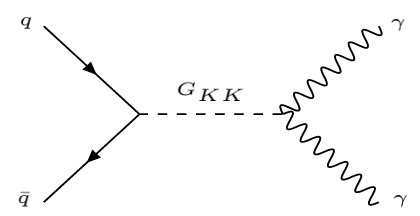
\includegraphics[scale=0.45]{figures/qqToGrav}
	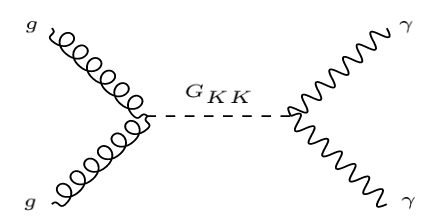
\includegraphics[scale=0.45]{figures/ggToGrav}
	\caption{Virtual graviton exchange in the diphoton ($\gamma\gamma$) channel through quark annihilation (left) and gluon fusion (right).}
	\label{signal_diagrams}
\end{figure}

The amplitude for any process involving virtual graviton exchange involves a sum over the \KK tower of \Gkk mass states, which can become divergent at high energies, so a cutoff scale needs to be introduced in order to regularize the cross section. Hence, the ADD model is an effective field theory valid only to some cutoff scale $\Lambda_{G}$. This ultraviolet cutoff scale is chosen to be the string scale \Ms~\cite{Han:1998sg}. This procedure results in a higher dimensional operator with coefficients suppressed by some mass scale~\cite{Gleisberg:2003ue}, which can be parametrized by $\etaG = \mathcal{F}/\Ms^4$, where $\mathcal{F}$ is a dimensionless parameter of order unity for which several conventions exist in the literature. We consider the conventions by Giudice, Rattazzi, and Wells (GRW)~\cite{Giudice:1998ck}; Han, Lykken, and Zhang (HLZ)~\cite{Han:1998sg}; and Hewett~\cite{Hewett:1998sn} expressed as:
\begin{equation}
	\label{eqn:add_f_conventions}
	\mathcal{F} = 
	\begin{cases} 
		1 \quad \text{(GRW)}, \\
		\log\left(\frac{\Ms^2}{\hat{s}} \right), \; \text{if} \; \nED = 2 \\ 
		\frac{2}{\nED - 2}, \; \text{if} \; \nED > 2 \\
		\pm\frac{2}{\pi} \quad \text{(Hewett)},
	\end{cases}
	\text{(HLZ)},
\end{equation}
where $\sqrt{\hat{s}}$, in the context of proton-proton collisions at the LHC, is the center-of-mass energy of the hard interaction from the colliding partons. \correction{In the HLZ convention only, $\mathcal{F}$ depends explicitly on \nED and, when $\nED=2$, there is an additional dependence on $\hat{s}$.}

\correction{Considering the interference between the ADD signal and the SM background, the total cross section depends on \etaG according to}
\begin{equation}
	\sigma_{\mathrm{total}} = \sigma_{\mathrm{SM}} + \etaG\, \sigma_{\mathrm{int}} + \etaG^2\, \sigma_{\mathrm{ADD}}
\end{equation}
where $\sigma_{\mathrm{SM}}$ is the cross section of the SM background of the desired processes, $\sigma_{\mathrm{ADD}}$ is the cross section of the pure ADD signal, and $\sigma_{\mathrm{int}}$ is the cross section arising from the interference between the two. The HLZ and GRW conventions interfere constructively, while the Hewett convention can interfere either constructively ($\mathcal{F} = +2/\pi$) or destructively ($\mathcal{F} = -2/\pi$).

For \KK gravitons in the {\TeVns} range, the branching ratios are nearly constant with graviton mass $m_G$ and the total decay width~\cite{Bijnens:2001gh,Tang:2012pv} can be expressed as
\begin{equation}
	\Gamma_{G} \simeq \frac{293m^3_{G}}{960\pi \Lambda^2_{G}}
\end{equation}
The main branching ratios for different SM particles are listed in Table~\ref{tab:grav_BR}. These are dominated by dijet ($gg$ and $q\bar{q}$) production, occurring about 2/3 of the time. Because the $\gamma\gamma$ and $ZZ$ modes contain identical particles, they acquire an additional factor of 1/2, as compared to the distinguishable $W^+W^-$ particles. \correction{The transverse mode of the $Z$ boson provides a contribution to the $ZZ$ branching ratio of the same amount as the $\gamma\gamma$ one; however, its longitudinal mode, acquired through the Higgs mechanism, yields one additional contribution to the $ZZ$ fraction not present for $\gamma\gamma$.} The ratio of the $gg$ to $\gamma\gamma$ branching ratios is 8, since there are 8 gluons but only a single $\gamma$.

\begin{table}[!htb]
	\centering
	\caption{The branching ratios for a massive graviton \Gkk decaying to SM particles with $q=u,d,c,s,b$ and $l=e,\mu$~\cite{Tang:2012pv}. \correction{The remaining 24 modes are split evenly among the 3 flavored neutrino-antineutrino pair and $\tau^+ \tau^-$ decay modes.}}
	\vspace{\baselineskip}
	\cmsTable{
	\begin{tabular}{rcccccccc}
	\hline \hline
	\vspace*{-4.0mm} & & & & & & & & \\
	\Gkk decay mode & $HH$   & $gg$   & $\gamma\gamma$ & $W^+W^-$ & $ZZ$   & $t\bar{t}$ & $q\bar{q}$ & $l^+ l^-$ \\
	Branching ratio &  2/293 & 96/293 & 12/293         & \correction{26/293}   & \correction{13/293} & \correction{18/293}     & 90/293     & 12/293 \vspace*{1.0mm}    \\
	\hline \hline
	\end{tabular}
	}
	\label{tab:grav_BR}
\end{table}

Searching for this ADD signal is favorable in the high-mass diphoton ($\gamma\gamma$) channel. Even though the \KK graviton branching ratio for dijets is dominant among all its decay channels, it suffers from a large background at the LHC. Further, the mass resolution for diphotons is superior to dijets, as provided by the CMS detector at the LHC and discussed in Chapter~\ref{ch:experiment}. Compared to the individual dilepton ($e^+e^-$ or $\mu^+\mu^-$) channels, the branching ratio to diphotons is twice as much. The graviton is a spin-2 particle, so its decay to leptons (spin-1/2) results in a restricted dilepton phase space, while photons are spin-1. Therefore, fermions, unlike photons, cannot be produced in $s$-wave scattering.

In the ADD model, the \Gkk modes are very finely spaced. Since the energy spacing between adjacent modes goes as $1/R$, they range from about 1\meV to about 100\MeV between $\nED=2$-7~\cite{Han:1998sg}. These individual decay modes are too fine to distinguish experimentally, limited by detector resolution. This leads to an effective nonresonant enhancement of the diphoton spectrum at high diphoton invariant mass (\mgg) resulting in a continuum spectrum of diphotons, rather than discrete resonances. Hence, the experimental signature is the nonresonant production of high-mass diphoton objects above the SM diphoton background.

This class of signatures described for the ADD model is by virtual graviton exchange. Since gravity couples to the stress-energy tensor, a graviton can be added to any fundamental SM vertex, e.g., the $s$-channel $q\bar{q}\gamma$ production vertex, allowing a search for direct graviton emission, where a graviton is emitted in the final state, e.g., in $q\bar{q} \to \gamma\Gkk$. These searches depend directly on \MD, and are complementary to the searches by virtual graviton exchange, depending on \Ms, which is expected to be on the order of \MD but may be different from it. An example search for direct graviton emission, as described by the ADD model, in the $\gamma\Gkk$ final state was recently performed by the CMS Collaboration~\cite{Sirunyan:2018dsf}. Interestingly, this model can also be probed by the possibility of microscopic black hole production when the collision energy exceeds \MD~\cite{Banks:1999gd,Dimopoulos:2001hw,Giddings:2001bu}. An example search for microscopic black hole production, as described by the ADD model, by the CMS Collaboration is presented in Ref.~\cite{Sirunyan:2018xwt}. This dissertation searches for signatures of ADD large extra dimensions by virtual graviton exchange in the high-mass diphoton channel using the CMS detector at the LHC.


\subsubsection{Limits on ADD Model Parameters}

No evidence has yet been seen for the existence of extra dimensions, but they have not been ruled out. Previous searches for extra-dimensional signals in the high-mass diphoton channel at collider experiments have been performed by the ATLAS~\cite{ATLAS:2011ab,Aad:2012cy,Aad:2015mna,Aaboud:2016tru,ATLAS-CONF-2016-059,Aaboud:2017yyg}, CMS~\cite{CMS-PAS-EXO-09-004,Chatrchyan:2011jx,Chatrchyan:2011fq,CMS-PAS-EXO-15-004,Khachatryan:2015qba,CMS-PAS-EXO-12-045,Khachatryan:2016yec,Khachatryan:2016hje,Sirunyan:2018wnk}, CDF~\cite{Aaltonen:2011xp}, and D0~\cite{Abazov:2010xh} Collaborations. The searches by the ATLAS and CMS experiments used proton-proton collisions at the LHC with center-of-mass energies $\sqrt{s} = 7,$ 8, and 13\TeV, while those by the CDF and D0 experiments used proton-antiproton collisions at the Tevatron with $\sqrt{s} = 1.96\TeV$. A summary of the extra-dimensional searches by the CMS experiment using $\sqrt{s} = 7$ and 8\TeV is presented by Landsberg in Ref.~\cite{Landsberg:2015pka}.

Searches for large extra dimensions arising from collider signals from virtual graviton effects at the LHC have been performed by the ATLAS and CMS Collaborations in the diphoton~\cite{Aaboud:2017yyg,Sirunyan:2018wnk}, dilepton~\cite{Aad:2014wca,Khachatryan:2014fba}, ditau~\cite{CMS-PAS-EXO-12-046}, and dijet~\cite{Sirunyan:2018wcm} channels. A summary of the corresponding searches in the high-mass diphoton channel by the CMS Collaboration is given in Table~\ref{tab:CMS_ADD_limits}.

% no \Kfactor is applied to the signal
\begin{table}[!htb]
	\centering
	\caption{\correction{A summary of the searches for large extra dimensions in the high-mass diphoton channel performed by the CMS Collaboration's Exotica (EXO) Physics Analysis Group prior to this dissertation.} The 95\% confidence level observed limits on \Ms are given, with the range depending on the model convention.}
	\vspace{\baselineskip}
	\begin{tabular}{cccccc}
	\hline \hline
	\vspace*{-4.5mm} & & & & & \\
	Search       & $\sqrt{s}$ & Data & Year & Limits on \Ms & Ref. \\
	\hline
	%CMS-EXO-09-004 & - & - & - & - & \cite{CMS-PAS-EXO-09-004} \\
	CMS-EXO-10-026 & 7\TeV & 36\pbinv & 2010 & 1.31-2.23\TeV & \cite{Chatrchyan:2011jx} \\
	CMS-EXO-11-038 & 7\TeV & 2.2\fbinv & 2011 & 2.28-3.50\TeV & \cite{Chatrchyan:2011fq} \\
	%CMS-EXO-17-017 & 13\TeV & 35.9\fbinv & 2016 & 5.6-9.7\TeV & \cite{Sirunyan:2018wnk} \\
	\hline \hline
	\end{tabular}
	\label{tab:CMS_ADD_limits}
\end{table}

The current best limits on the ADD model of large extra dimensions arising from collider signals from virtual graviton effects are due to the CMS dijet angular search~\cite{Sirunyan:2018wcm}. This search used data corresponding to 35.9\fbinv with $\sqrt{s} = 13\TeV$. The 95\% confidence level limits on \Ms range between 8.5-12.0\TeV, depending on the model convention. The use of the dijet angular variable provides superior signal sensitivity than simply considering only the dijet invariant mass. In the diphoton channel, ATLAS sets 95\% confidence level limits on \Ms between 5.7-8.1\TeV using 37\fbinv with $\sqrt{s} = 13\TeV$~\cite{Aaboud:2017yyg}. This dissertation searches in the CMS high-mass diphoton channel using 35.9\fbinv with $\sqrt{s} = 13\TeV$~\cite{Sirunyan:2018wnk} and aims to extend these results.


\section{Organization of Dissertation}

The remainder of this dissertation is organized as follows. \correction{The experimental apparatus used in this large-extra dimensional search is the combination of the LHC and CMS detector}, as described in Chapter~\ref{ch:experiment}. Event reconstruction and selection within the CMS detector, with an emphasis on photon reconstruction and diphoton selection, are detailed in Chapter~\ref{ch:event_selection}. Chapter~\ref{ch:background} presents the background determination for this nonresonant diphoton search. The ADD large extra-dimensional signal is simulated according to the methods of Chapter~\ref{ch:signal}. Sources of systematic uncertainty are discussed in Chapter~\ref{ch:systematics}, and the results are presented in Chapter~\ref{ch:results}.



